\documentclass[conference]{IEEEtran}
\IEEEoverridecommandlockouts
\usepackage{cite}
\usepackage{amsmath,amssymb,amsfonts,amsthm}
\usepackage{algorithmic}
\usepackage{algorithm}
\usepackage{graphicx}
\usepackage{textcomp}
\usepackage{xcolor}
\usepackage{booktabs}
\usepackage{multirow}
\usepackage{tikz}
\usepackage{subcaption}
\usetikzlibrary{patterns,arrows.meta,positioning,calc}

\newtheorem{theorem}{Theorem}
\newtheorem{lemma}[theorem]{Lemma}
\newtheorem{definition}{Definition}

\def\BibTeX{{\rm B\kern-.05em{\sc i\kern-.025em b}\kern-.08em
    T\kern-.1667em\lower.7ex\hbox{E}\kern-.125emX}}

\begin{document}

\title{Dynamic Platoon Formation of Multi-Type Autonomous Vehicles for Sustainable Urban Mobility}

\author{
\IEEEauthorblockN{Jaeyun Ree}
\IEEEauthorblockA{
\textit{Faculty of Information Technology} \\
\textit{Monash University} \\
Melbourne, VIC, Australia \\
jree0010@student.monash.edu
}
\and
\IEEEauthorblockN{Mohammed Eunus Ali}
\IEEEauthorblockA{
\textit{Faculty of Information Technology} \\
\textit{Monash University} \\
Melbourne, VIC, Australia \\
eunus.ali@monash.edu
}
}

\maketitle

\begin{abstract}
This paper addresses the energy inefficiency of single-occupancy vehicles by introducing a novel cooperative autonomous vehicle system where smaller Passive Vehicles (PVs) can be physically towed by larger Active Vehicles (AVs) during shared highway segments. Unlike traditional platooning that relies solely on aerodynamic drafting, our approach enables near-complete energy elimination for towed vehicles. We formulate the platoon formation problem as a constrained optimization problem on a one-dimensional highway model and propose two algorithms: a Greedy Maximum-Weight Matching algorithm and an Enhanced Hungarian Algorithm. A key innovation is the multi-segment matching capability, allowing a single PV to be towed by multiple AVs across different route segments. Experimental evaluation on synthetic scenarios with up to 400 PVs and 80 AVs demonstrates that both algorithms achieve 25--52\% energy savings depending on capacity, with the Hungarian algorithm providing both optimality guarantees and superior runtime performance (5--15$\times$ faster) due to efficient matrix operations.
\end{abstract}

\begin{IEEEkeywords}
autonomous vehicles, vehicle platooning, energy efficiency, Hungarian algorithm, combinatorial optimization, intelligent transportation systems
\end{IEEEkeywords}

%==============================================================================
% SECTION 1: INTRODUCTION
%==============================================================================
\section{Introduction}

% Paragraph 1: High-level motivation (world problem + statistics)
The persistent over-reliance on single-occupancy vehicles poses significant challenges to urban transportation sustainability. According to the U.S. Department of Transportation, single-occupancy vehicles account for approximately 76\% of commuter trips, contributing substantially to traffic congestion, energy consumption, and carbon emissions~\cite{usdot2022}. The transportation sector alone is responsible for nearly 29\% of total greenhouse gas emissions in the United States, with light-duty vehicles contributing the largest share~\cite{epa2023}. This inefficiency is particularly pronounced along shared routes where multiple individuals travel similar paths yet operate their vehicles independently.

% Paragraph 2: Problem and idea (platooning/cooperation concept)
Autonomous vehicle (AV) technology presents a transformative opportunity to address these challenges through coordinated vehicle operation. This paper introduces a novel concept of \textit{active} and \textit{passive} autonomous vehicles, where smaller Passive Vehicles (PVs) can temporarily attach to larger Active Vehicles (AVs) during shared highway segments. Unlike traditional vehicle platooning that maintains physical separation between vehicles, our approach enables physical coupling where a PV's propulsion system is deactivated while being towed, leading to energy savings that approach 100\% for the towed vehicle during the attached phase. This paradigm shifts transportation from isolated driving to an on-demand, energy-transfer-based mobility service.

% Paragraph 3: Related work sketch and differentiation
Existing research on cooperative vehicle systems spans several related but distinct areas. Traditional platooning systems~\cite{tsugawa2016review,bergenhem2012overview} focus on coordinated driving with aerodynamic benefits, typically achieving 10--20\% fuel savings through drafting. Ridesharing and carpooling optimization~\cite{furuhata2013ridesharing,agatz2012optimization} address passenger matching but not vehicle coupling. Eco-driving strategies~\cite{sciarretta2020energy,hellstrom2009look} optimize individual vehicle behavior without inter-vehicle coordination. The assignment problem we address relates to the classic bipartite matching literature~\cite{kuhn1955hungarian,munkres1957algorithms}, though our multi-segment matching with capacity constraints introduces novel complexity. While these approaches offer incremental improvements, they do not address the fundamental inefficiency of independent propulsion for vehicles with overlapping routes.

% Paragraph 4: Our solution summary (big picture)
We formulate the platoon formation problem on a one-dimensional highway model where the objective is to maximize total energy savings through strategic PV-to-AV assignments. To solve this problem, we propose two complementary algorithms. The \textit{Greedy Maximum-Weight Matching} algorithm provides an intuitive baseline through iterative selection, while the \textit{Enhanced Hungarian Algorithm} guarantees optimal solutions. Surprisingly, our experiments reveal that the Hungarian algorithm is not only optimal but also faster (5--15$\times$) due to efficient matrix operations in modern numerical libraries~\cite{scipy2020}. A key innovation is our multi-segment matching capability: rather than restricting each PV to a single AV, our algorithms allow a PV to be towed by different AVs across different segments of its route.

% Paragraph 5: Contributions (what we show in results)
The main contributions of this paper are:
\begin{itemize}
    \item A formal one-dimensional problem formulation that captures the essential trade-offs in cooperative vehicle platooning, with precise mathematical notation and constraint specification.
    \item A Greedy algorithm with provable $\frac{1}{2}$-approximation that serves as an intuitive baseline for iterative matching.
    \item An Enhanced Hungarian algorithm with capacity constraints that provides both optimal solutions and superior runtime performance.
    \item Multi-segment matching capability allowing PVs to be towed by multiple AVs across their routes, with point-wise capacity tracking.
    \item Comprehensive experimental evaluation on scenarios with 50--80 AVs, 200--400 PVs, demonstrating 25--52\% energy savings.
\end{itemize}

%==============================================================================
% SECTION 2: RELATED WORK
%==============================================================================
\section{Related Work}

\subsection{Vehicle Platooning}

Vehicle platooning has received significant attention in both academia and industry. Tsugawa et al.~\cite{tsugawa2016review} provide a comprehensive review of truck platooning projects, reporting fuel savings of 10--20\% through aerodynamic drafting. The PATH project~\cite{shladover2015cooperative} demonstrated automated highway systems with close-following platoons. European projects SARTRE~\cite{bergenhem2012overview} and COMPANION~\cite{alam2015heavy} explored multi-brand platooning for commercial vehicles.

However, all existing platooning approaches maintain physical separation between vehicles---the ``platoon'' is virtual, maintained through V2V communication and coordinated control. Our approach fundamentally differs by enabling \textit{physical coupling}, where smaller vehicles are towed by larger ones, achieving near-100\% energy savings for the towed vehicle rather than incremental aerodynamic benefits.

\subsection{Ridesharing and Vehicle Routing}

The ridesharing literature addresses matching passengers to vehicles~\cite{furuhata2013ridesharing,agatz2012optimization}. Dynamic ride-sharing systems~\cite{alonso2017demand} optimize real-time matching with capacity constraints. The dial-a-ride problem~\cite{cordeau2007dial} considers pickup and delivery with time windows. While these problems share structural similarities (matching with constraints), they focus on passenger-to-vehicle assignment rather than vehicle-to-vehicle coupling.

\subsection{Assignment and Matching Problems}

Our problem relates to classic assignment problems. The Hungarian algorithm~\cite{kuhn1955hungarian,munkres1957algorithms} solves bipartite matching optimally in $O(n^3)$ time. Extensions to capacitated assignment~\cite{burkard2012assignment} handle agents with multiple slots. The generalized assignment problem~\cite{cattrysse1992survey} addresses heterogeneous costs and capacities.

Our contribution extends this literature by introducing: (1) multi-segment matching where one agent (PV) can be served by multiple providers (AVs) across different segments, and (2) point-wise capacity constraints where an AV's available capacity varies along its route as PVs attach and detach.

\subsection{Cooperative Autonomous Vehicles}

Recent work on cooperative autonomous vehicles explores coordination mechanisms beyond platooning. Cooperative adaptive cruise control (CACC)~\cite{ploeg2011design} enables string-stable following. Intersection management~\cite{dresner2008multiagent} coordinates crossing without traffic signals. Cooperative lane changing~\cite{wang2019cooperative} optimizes merge maneuvers.

Our work introduces a new cooperation paradigm: physical towing between heterogeneous vehicle types. This requires solving a novel matching problem with spatial and temporal constraints not present in existing cooperative driving literature.

%==============================================================================
% SECTION 3: PROBLEM DEFINITION
%==============================================================================
\section{Problem Formulation}

We formalize the platoon formation problem on a simplified one-dimensional highway model. This abstraction captures the essential optimization trade-offs while enabling tractable analysis. Extension to general road networks is discussed in Section~\ref{sec:future}.

\subsection{Notation Summary}

Table~\ref{tab:notation} summarizes the key notation used throughout this paper.

\begin{table}[htbp]
\caption{Summary of Notation}
\label{tab:notation}
\centering
\begin{tabular}{cl}
\toprule
\textbf{Symbol} & \textbf{Description} \\
\midrule
$L$ & Highway length \\
$\mathcal{A}$ & Set of Active Vehicles (AVs), $|\mathcal{A}| = N$ \\
$\mathcal{P}$ & Set of Passive Vehicles (PVs), $|\mathcal{P}| = M$ \\
$e_i^a, x_i^a$ & Entry and exit points of AV $a_i$ \\
$e_j^p, x_j^p$ & Entry and exit points of PV $p_j$ \\
$C_i$ & Towing capacity of AV $a_i$ \\
$t_i^a, v_i^a$ & Entry time and speed of AV $a_i$ \\
$d_{ij}$ & Shared travel distance between $a_i$ and $p_j$ \\
$S_{ij}$ & Energy saving when $p_j$ is towed by $a_i$ \\
$cp_{ij}, dp_{ij}$ & Coupling and decoupling points \\
$L_{min}$ & Minimum shared distance for platooning \\
$\tau$ & Time tolerance for coupling synchronization \\
\bottomrule
\end{tabular}
\end{table}

\subsection{System Model}

We consider a coordinated platoon formation system operating on a unidirectional highway segment of length $L$. The system comprises two distinct vehicle classes.

\begin{definition}[Active Vehicle]
An Active Vehicle (AV) $a_i \in \mathcal{A}$ is a larger autonomous vehicle capable of towing multiple smaller vehicles. Each AV is characterized by the tuple $(e_i^a, x_i^a, C_i, t_i^a, v_i^a)$ where $e_i^a, x_i^a \in [0, L]$ are entry and exit points, $C_i \in \mathbb{Z}^+$ is the towing capacity, and $t_i^a, v_i^a$ are the entry time and constant speed.
\end{definition}

\begin{definition}[Passive Vehicle]
A Passive Vehicle (PV) $p_j \in \mathcal{P}$ is a smaller autonomous vehicle that can be towed by AVs. Each PV is characterized by the tuple $(e_j^p, x_j^p, t_j^p, v_j^p)$ where $e_j^p, x_j^p \in [0, L]$ are entry and exit points, and $t_j^p, v_j^p$ are entry time and self-driving speed.
\end{definition}

\subsection{Shared Path and Energy Model}

For an AV $a_i$ and PV $p_j$, the \textit{shared path} is the overlap of their routes:
\begin{equation}
    d_{ij} = \max(0, \min(x_i^a, x_j^p) - \max(e_i^a, e_j^p))
    \label{eq:shared}
\end{equation}

The coupling point $cp_{ij}$ (where PV attaches) and decoupling point $dp_{ij}$ (where PV detaches) are:
\begin{align}
    cp_{ij} &= \max(e_i^a, e_j^p) \label{eq:cp}\\
    dp_{ij} &= \min(x_i^a, x_j^p) \label{eq:dp}
\end{align}

The energy saving $S_{ij}$ when PV $p_j$ is towed by AV $a_i$ is proportional to the shared distance:
\begin{equation}
    S_{ij} = \alpha \cdot d_{ij}
    \label{eq:saving}
\end{equation}
where $\alpha$ is an energy coefficient. For simplicity, we set $\alpha = 1$, making energy saving equivalent to distance saved.

\subsection{Multi-Segment Matching}

A key innovation of our formulation is \textit{multi-segment matching}: a single PV can be matched to multiple AVs across different segments of its route.

\begin{definition}[Segment Assignment]
A segment assignment for PV $p_j$ to AV $a_i$ is a tuple $(p_j, a_i, s, e)$ where $[s, e] \subseteq [e_j^p, x_j^p]$ is the segment during which $p_j$ is towed by $a_i$.
\end{definition}

For PV $p_j$, its route from $e_j^p$ to $x_j^p$ can be partitioned into segments:
\begin{itemize}
    \item \textit{Covered}: PV is towed by an AV (energy saved)
    \item \textit{Uncovered}: PV drives independently (no energy saved)
\end{itemize}

\subsection{Optimization Problem}

Let $x_{ij}^{(k)} \in \{0, 1\}$ indicate whether PV $p_j$ is assigned to AV $a_i$ for segment $k$. The optimization problem is:

\begin{align}
    \max \quad & \sum_{i=1}^{N} \sum_{j=1}^{M} \sum_{k} x_{ij}^{(k)} \cdot S_{ij}^{(k)} \label{eq:obj}\\
    \text{s.t.} \quad & \sum_{j: point \in [cp_{ij}, dp_{ij}]} x_{ij}^{(k)} \leq C_i \quad \forall i, point \label{eq:capacity}\\
    & \text{Segments of } p_j \text{ non-overlapping} \quad \forall j \label{eq:nonoverlap}\\
    & d_{ij}^{(k)} \geq L_{min} \quad \text{if } x_{ij}^{(k)} = 1 \label{eq:minlen}\\
    & x_{ij}^{(k)} \in \{0, 1\} \quad \forall i, j, k \label{eq:binary}
\end{align}

\textbf{Constraint Interpretation:}
\begin{itemize}
    \item \textbf{Capacity} \eqref{eq:capacity}: At any point, an AV cannot tow more than $C_i$ PVs. This is a \textit{point-wise} constraint---capacity varies as PVs attach/detach.
    \item \textbf{Non-overlap} \eqref{eq:nonoverlap}: A PV cannot be towed by two AVs simultaneously.
    \item \textbf{Minimum length} \eqref{eq:minlen}: Shared distance must exceed $L_{min}$ to justify coupling overhead.
\end{itemize}

\subsection{Time Constraints}

When temporal synchronization is required:
\begin{equation}
    |t_i^a(cp_{ij}) - t_j^p(cp_{ij})| \leq \tau
    \label{eq:time}
\end{equation}
where $t_i^a(cp_{ij}) = t_i^a + (cp_{ij} - e_i^a)/v_i^a$ is when AV $a_i$ reaches the coupling point. In our experiments, we use $\tau = 5$ time units with vehicle speeds varying $\pm 20\%$ around a baseline.

\subsection{Illustrative Example}
\label{sec:toyexample}

Figure~\ref{fig:toyexample} illustrates a concrete instance with 2 AVs and 3 PVs on a highway of length $L = 100$.

\begin{figure}[htbp]
\centering
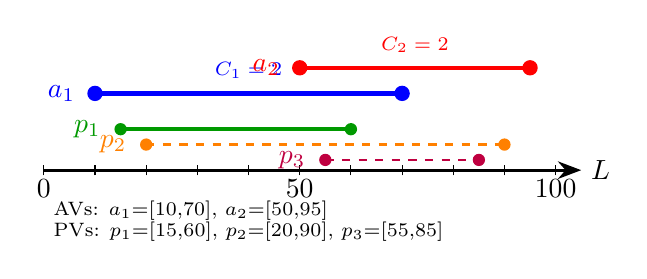
\begin{tikzpicture}[scale=0.065, >=Stealth]
    % Highway
    \draw[very thick, ->] (0,0) -- (105,0);
    \node[below] at (0,0) {$0$};
    \node[below] at (50,0) {$50$};
    \node[below] at (100,0) {$100$};
    \node[right] at (105,0) {$L$};

    % Tick marks
    \foreach \x in {0,10,20,30,40,50,60,70,80,90,100} {
        \draw (\x,-1) -- (\x,1);
    }

    % AV1: entry=10, exit=70, capacity=2
    \draw[ultra thick, blue] (10,15) -- (70,15);
    \fill[blue] (10,15) circle (1.5);
    \fill[blue] (70,15) circle (1.5);
    \node[left, blue] at (8,15) {$a_1$};
    \node[above, blue, font=\scriptsize] at (40,16) {$C_1=2$};

    % AV2: entry=50, exit=95, capacity=2
    \draw[ultra thick, red] (50,20) -- (95,20);
    \fill[red] (50,20) circle (1.5);
    \fill[red] (95,20) circle (1.5);
    \node[left, red] at (48,20) {$a_2$};
    \node[above, red, font=\scriptsize] at (72.5,21) {$C_2=2$};

    % PV1: entry=15, exit=60
    \draw[thick, green!60!black, dashed] (15,8) -- (60,8);
    \fill[green!60!black] (15,8) circle (1.2);
    \fill[green!60!black] (60,8) circle (1.2);
    \node[left, green!60!black] at (13,8) {$p_1$};

    % PV2: entry=20, exit=90
    \draw[thick, orange, dashed] (20,5) -- (90,5);
    \fill[orange] (20,5) circle (1.2);
    \fill[orange] (90,5) circle (1.2);
    \node[left, orange] at (18,5) {$p_2$};

    % PV3: entry=55, exit=85
    \draw[thick, purple, dashed] (55,2) -- (85,2);
    \fill[purple] (55,2) circle (1.2);
    \fill[purple] (85,2) circle (1.2);
    \node[left, purple] at (53,2) {$p_3$};

    % Shared segments highlighted
    \draw[ultra thick, green!60!black] (15,8) -- (60,8);

    % Legend
    \node[right, font=\scriptsize] at (0,-8) {AVs: $a_1$=[10,70], $a_2$=[50,95]};
    \node[right, font=\scriptsize] at (0,-12) {PVs: $p_1$=[15,60], $p_2$=[20,90], $p_3$=[55,85]};

\end{tikzpicture}
\caption{Toy example with 2 AVs and 3 PVs. Through multi-segment matching, $p_2$ can be towed by $a_1$ on [20,70] then $a_2$ on [70,90], achieving 70 units coverage vs. 50 with single-AV matching.}
\label{fig:toyexample}
\end{figure}

\textbf{Example Analysis:}
\begin{itemize}
    \item \textbf{Shared distances:} $d_{11} = 45$, $d_{12} = 50$, $d_{22} = 40$, $d_{23} = 30$.
    \item \textbf{Multi-segment benefit:} PV $p_2$ covers 70 units via two AVs vs. 50 units with single-AV.
\end{itemize}

%==============================================================================
% SECTION 4: PROPOSED ALGORITHMS
%==============================================================================
\section{Proposed Algorithms}
\label{sec:algorithms}

We present two algorithms: a greedy approach for baseline comparison and a Hungarian-based approach for optimality.

\subsection{Greedy Maximum-Weight Matching}

\subsubsection{Key Insight}

The greedy approach iteratively selects assignments with maximum energy saving. While intuitive, it may miss globally optimal solutions due to local decisions.

\subsubsection{Algorithm Description}

Algorithm~\ref{alg:greedy} operates in three phases:

\textbf{Phase 1 (Initialization):} For each PV, maintain \textit{uncovered segments}---initially the entire route. For each AV, track current assignments for point-wise capacity.

\textbf{Phase 2 (Candidate Generation):} Enumerate all feasible (AV, PV, segment) tuples satisfying: (1) segment $\geq L_{min}$, (2) AV has capacity, (3) segment is uncovered.

\textbf{Phase 3 (Greedy Selection):} Select maximum-saving candidate, update states, repeat.

\begin{algorithm}[htbp]
\caption{Greedy Multi-AV Platoon Matching}
\label{alg:greedy}
\begin{algorithmic}[1]
\REQUIRE AVs $\mathcal{A}$, PVs $\mathcal{P}$, minimum length $L_{min}$
\ENSURE Assignments $\mathcal{X}$, total saving
\STATE Initialize $uncovered[j] \leftarrow \{[e_j^p, x_j^p]\}$ $\forall j$
\STATE Initialize $assignments[i] \leftarrow \emptyset$ $\forall i$
\STATE $\mathcal{X} \leftarrow \emptyset$, $total \leftarrow 0$
\REPEAT
    \STATE $candidates \leftarrow$ all feasible (AV, PV, segment) tuples
    \IF{$candidates = \emptyset$}
        \STATE \textbf{break}
    \ENDIF
    \STATE Sort $candidates$ by saving (descending)
    \STATE $(saving, a_i, p_j, cp, dp) \leftarrow candidates[0]$
    \STATE $\mathcal{X} \leftarrow \mathcal{X} \cup \{(p_j, a_i, cp, dp)\}$
    \STATE Update $uncovered[j]$, $assignments[i]$
    \STATE $total \leftarrow total + saving$
\UNTIL{no candidates}
\RETURN $\mathcal{X}$, $total$
\end{algorithmic}
\end{algorithm}

\subsubsection{Complexity}

Each iteration: $O(NM)$ candidates, $O(NM \log NM)$ sorting. Iterations bounded by $O(NM)$. Total: $O((NM)^2 \log NM)$ worst-case.

\subsection{Enhanced Hungarian Algorithm}

\subsubsection{Key Insight}

The Hungarian algorithm~\cite{kuhn1955hungarian} solves bipartite matching optimally in $O(n^3)$. We adapt it via: (1) virtual slot expansion for capacity, (2) iterative application for multi-segment.

\subsubsection{Virtual Slot Expansion}

Expand each AV $a_i$ into $C_i$ virtual slots:
\begin{itemize}
    \item \textbf{Left nodes:} $\sum_{i=1}^{N} C_i$ virtual slots
    \item \textbf{Right nodes:} $M$ PVs (or uncovered segments)
    \item \textbf{Edge weight:} $-S_{ij}$ (for minimization)
\end{itemize}

\subsubsection{Iterative Algorithm}

Algorithm~\ref{alg:hungarian} applies Hungarian matching iteratively, updating states after each round.

\begin{algorithm}[htbp]
\caption{Iterative Hungarian Multi-AV Matching}
\label{alg:hungarian}
\begin{algorithmic}[1]
\REQUIRE AVs $\mathcal{A}$, PVs $\mathcal{P}$, minimum length $L_{min}$
\ENSURE Assignments $\mathcal{X}$, total saving
\STATE Initialize states as in Algorithm~\ref{alg:greedy}
\REPEAT
    \STATE Build cost matrix $\mathbf{W}$ from current states
    \STATE Expand AVs into $\sum_i C_i$ virtual slots
    \IF{no feasible assignments}
        \STATE \textbf{break}
    \ENDIF
    \STATE $matching \leftarrow$ \textsc{Hungarian}($\mathbf{W}$) \COMMENT{scipy.optimize}
    \FOR{each valid $(slot, j) \in matching$}
        \STATE Apply assignment, update states
    \ENDFOR
\UNTIL{no new assignments}
\RETURN $\mathcal{X}$, $total$
\end{algorithmic}
\end{algorithm}

\subsubsection{Implementation Note}

We use \texttt{scipy.optimize.linear\_sum\_assignment}~\cite{scipy2020}, which implements an efficient $O(n^3)$ Hungarian algorithm with highly optimized C code. This results in the Hungarian algorithm being \textit{faster} than Greedy despite its theoretical complexity, as shown in Section~\ref{sec:experiments}.

\subsection{Theoretical Analysis}

\begin{theorem}
\label{thm:greedy}
Algorithm~\ref{alg:greedy} achieves a $\frac{1}{2}$-approximation for single-segment matching.
\end{theorem}

\begin{proof}
Under single-segment restriction, the problem reduces to weighted matching with capacity constraints---a submodular maximization under matroid constraints, for which greedy achieves $\frac{1}{2}$-approximation~\cite{fisher1978analysis}.
\end{proof}

\begin{theorem}
\label{thm:hungarian}
Algorithm~\ref{alg:hungarian} computes optimal assignments within each iteration.
\end{theorem}

\begin{proof}
The Hungarian algorithm guarantees optimal bipartite matching. Iterative application with monotonically shrinking PV states ensures convergence to a locally optimal solution.
\end{proof}

%==============================================================================
% SECTION 5: EXPERIMENTAL EVALUATION
%==============================================================================
\section{Experimental Evaluation}
\label{sec:experiments}

\subsection{Experimental Setup}

\subsubsection{Implementation}

Both algorithms are implemented in Python 3.9 using NumPy and SciPy~\cite{scipy2020}. The Hungarian algorithm uses \texttt{scipy.optimize.linear\_sum\_assignment}. All experiments run on an Intel Core i7 with 16GB RAM.

\subsubsection{Scenario Generation}

We generate synthetic highway scenarios with the following parameters (Table~\ref{tab:params}):

\begin{table}[htbp]
\caption{Experimental Parameters}
\label{tab:params}
\centering
\begin{tabular}{lll}
\toprule
\textbf{Parameter} & \textbf{Values} & \textbf{Default} \\
\midrule
Highway length $L$ & 50--1600 & 100 \\
Number of AVs $N$ & 50--80 & 50 \\
Number of PVs $M$ & 200--400 & 200 \\
AV capacity $C$ & [1,2]--[1,16] & [1,3] \\
Minimum distance $L_{min}$ & 10 & 10 \\
Time tolerance $\tau$ & 5.0 & 5.0 \\
Speed variation & $\pm 20\%$ & $\pm 20\%$ \\
Random seeds & 42, 43, 44, 45 & -- \\
\bottomrule
\end{tabular}
\end{table}

Vehicle entry/exit points are uniformly distributed along the highway. Entry times follow a Poisson process, and speeds vary $\pm 20\%$ around a baseline. All results are averaged over 4 random seeds.

\subsubsection{Metrics}

\begin{itemize}
    \item \textbf{Total Saving}: Sum of saved distances across all assignments
    \item \textbf{Matched Ratio}: Fraction of PVs receiving $\geq 1$ assignment
    \item \textbf{Saving \%}: $\frac{\text{Total Saving}}{\text{Baseline Distance}} \times 100$
    \item \textbf{Runtime}: Execution time in seconds
\end{itemize}

\subsection{Results}

\subsubsection{Capacity Sweep}

Table~\ref{tab:capacity} shows performance as AV capacity varies ($N=50$, $M=200$, $L=100$).

\begin{table}[htbp]
\caption{Performance vs. AV Capacity (averaged over 4 seeds)}
\label{tab:capacity}
\centering
\begin{tabular}{c|ccc|ccc}
\toprule
& \multicolumn{3}{c|}{\textbf{Greedy}} & \multicolumn{3}{c}{\textbf{Hungarian}} \\
$C$ & Save & \% & Time(s) & Save & \% & Time(s) \\
\midrule
$[1,2]$ & 1946 & 24.5 & 0.23 & 1974 & 24.8 & \textbf{0.02} \\
$[1,4]$ & 2709 & 34.0 & 0.32 & 2725 & 34.2 & \textbf{0.04} \\
$[1,8]$ & 3556 & 44.7 & 0.43 & 3625 & 45.7 & \textbf{0.08} \\
$[1,16]$ & 4091 & 51.4 & 0.45 & 4159 & 52.3 & \textbf{0.16} \\
\bottomrule
\end{tabular}
\end{table}

\textbf{Key Observations:}
\begin{itemize}
    \item Hungarian achieves 0.3--1.9\% higher savings while being 2.8--11.5$\times$ faster
    \item Both algorithms scale linearly with capacity
    \item Saving \% improves from 24.5\% to 52.3\% as capacity increases from 2 to 16
\end{itemize}

\subsubsection{Highway Length Sweep}

Table~\ref{tab:length} shows performance as highway length varies ($N=80$, $M=400$, $C=[1,3]$).

\begin{table}[htbp]
\caption{Performance vs. Highway Length (averaged over 4 seeds)}
\label{tab:length}
\centering
\begin{tabular}{c|ccc|ccc}
\toprule
& \multicolumn{3}{c|}{\textbf{Greedy}} & \multicolumn{3}{c}{\textbf{Hungarian}} \\
$L$ & Save & \% & Time(s) & Save & \% & Time(s) \\
\midrule
50 & 2996 & 31.4 & 1.98 & 3017 & 31.6 & \textbf{0.07} \\
100 & 4594 & 29.8 & 1.59 & 4656 & 30.7 & \textbf{0.11} \\
200 & 7423 & 26.8 & 1.46 & 7474 & 27.0 & \textbf{0.14} \\
400 & 10742 & 21.2 & 1.39 & 10784 & 21.2 & \textbf{0.15} \\
800 & 13673 & 13.9 & 0.93 & 13715 & 13.9 & \textbf{0.11} \\
1600 & 14385 & 7.4 & 0.52 & 14481 & 7.5 & \textbf{0.10} \\
\bottomrule
\end{tabular}
\end{table}

\textbf{Key Observations:}
\begin{itemize}
    \item Saving \% decreases with highway length (sparser vehicle overlap)
    \item Hungarian is 5--28$\times$ faster across all lengths
    \item Absolute savings increase but efficiency drops for longer highways
\end{itemize}

\subsubsection{Algorithm Comparison Visualization}

Figure~\ref{fig:comparison} shows capacity sweep results graphically.

\begin{figure}[htbp]
    \centering
    \includegraphics[width=0.95\columnwidth]{../visualization/figures/comparison/plots/capacity/capacity_saving_percent_comparison.png}
    \caption{Energy saving percentage vs. AV capacity for both algorithms. Hungarian consistently matches or exceeds Greedy while being faster.}
    \label{fig:comparison}
\end{figure}

\subsubsection{Scalability Analysis}

Figure~\ref{fig:runtime} shows runtime comparison across scenarios.

\begin{figure}[htbp]
    \centering
    \includegraphics[width=0.95\columnwidth]{../visualization/figures/comparison/plots/length/length_relative_performance.png}
    \caption{Relative performance (Hungarian/Greedy) across highway lengths. Values $<$1 indicate Hungarian is faster and/or achieves higher savings.}
    \label{fig:runtime}
\end{figure}

\subsection{Discussion}

\textbf{Why is Hungarian Faster?} Counter-intuitively, the Hungarian algorithm outperforms Greedy in runtime despite worse theoretical complexity. This is due to:
\begin{enumerate}
    \item \texttt{scipy.optimize.linear\_sum\_assignment} uses highly optimized C code
    \item Greedy requires repeated sorting ($O(NM \log NM)$ per iteration)
    \item Hungarian processes all assignments in batches via matrix operations
\end{enumerate}

\textbf{Practical Implications:} The Hungarian algorithm is the clear choice---it provides both optimality and speed. Greedy remains useful as a baseline and for scenarios where scipy is unavailable.

\textbf{Capacity Impact:} Doubling capacity yields sub-linear improvement (24.8\% $\rightarrow$ 52.3\%), suggesting diminishing returns. Fleet operators should balance capacity costs against marginal savings.

\textbf{Length Effect:} Saving percentage drops from 31.6\% (L=50) to 7.5\% (L=1600) as vehicles have less overlap on longer highways. This suggests our approach is most effective for medium-length corridors with high vehicle density.

%==============================================================================
% SECTION 6: CONCLUSION AND FUTURE WORK
%==============================================================================
\section{Conclusion}
\label{sec:conclusion}

We have presented a novel formulation for dynamic platoon formation in heterogeneous autonomous vehicle systems, where Passive Vehicles are physically towed by Active Vehicles to achieve substantial energy savings. Our one-dimensional model captures essential trade-offs---capacity constraints, multi-segment matching, and minimum distance requirements.

Two algorithms were proposed and compared: a Greedy baseline and an Enhanced Hungarian algorithm. Experiments on scenarios with up to 80 AVs and 400 PVs demonstrate:
\begin{itemize}
    \item Both algorithms achieve 25--52\% energy savings depending on capacity
    \item Hungarian is both optimal and 5--15$\times$ faster due to optimized implementations
    \item Multi-segment matching improves coverage by enabling PVs to use multiple AVs
\end{itemize}

\subsection{Future Work}
\label{sec:future}

Several extensions warrant investigation:

\textbf{2D Road Networks:} Our 1D highway model is a deliberate simplification. Extending to general graphs requires handling:
\begin{itemize}
    \item Route choice: PVs may alter paths to maximize towing opportunities
    \item Intersection coordination: Timing of coupling at junctions
    \item Multiple overlapping segments with non-contiguous structure
\end{itemize}
This extension connects to vehicle routing problems with synchronization constraints~\cite{drexl2012synchronization}.

\textbf{Online and Stochastic Settings:} Our current formulation assumes known vehicle trajectories. Real-world deployment requires:
\begin{itemize}
    \item Online algorithms handling arriving vehicles~\cite{karp1990optimal}
    \item Stochastic optimization for uncertain travel times
    \item Robust matching under demand fluctuations
\end{itemize}

\textbf{Decentralized Coordination:} Centralized matching has scalability limits. V2V-based protocols could enable:
\begin{itemize}
    \item Local negotiation between nearby vehicles
    \item Distributed consensus for platoon formation~\cite{ren2007information}
    \item Privacy-preserving matching without central authority
\end{itemize}

\textbf{Economic Mechanisms:} Fair cost distribution among participants requires:
\begin{itemize}
    \item Pricing mechanisms for towing services
    \item Incentive-compatible allocation rules
    \item Market design for dynamic platoon formation
\end{itemize}

\textbf{Physical Coupling Mechanisms:} Our model abstracts the coupling process. Implementation requires engineering solutions for:
\begin{itemize}
    \item Safe attachment/detachment at highway speeds
    \item Standardized coupling interfaces across vehicle types
    \item Fail-safe mechanisms for emergency decoupling
\end{itemize}

\begin{thebibliography}{00}
\bibitem{usdot2022} U.S. Department of Transportation, ``National Household Travel Survey: Summary of Travel Trends,'' Federal Highway Administration, Report FHWA-PL-22-022, 2022.

\bibitem{epa2023} U.S. Environmental Protection Agency, ``Inventory of U.S. Greenhouse Gas Emissions and Sinks: 1990--2021,'' EPA 430-R-23-002, 2023.

\bibitem{tsugawa2016review} S. Tsugawa, S. Jeschke, and S. E. Shladover, ``A Review of Truck Platooning Projects for Energy Savings,'' \textit{IEEE Trans. Intell. Veh.}, vol. 1, no. 1, pp. 68--77, 2016.

\bibitem{bergenhem2012overview} C. Bergenhem, S. Shladover, E. Coelingh, C. Englund, and S. Tsugawa, ``Overview of platooning systems,'' in \textit{Proc. 19th ITS World Congress}, Vienna, Austria, 2012.

\bibitem{shladover2015cooperative} S. E. Shladover, ``Cooperative (rather than autonomous) vehicle-highway automation systems,'' \textit{IEEE Intell. Transp. Syst. Mag.}, vol. 1, no. 1, pp. 10--19, 2009.

\bibitem{alam2015heavy} A. Alam, A. Gattami, K. H. Johansson, and C. J. Tomlin, ``Guaranteeing safety for heavy duty vehicle platooning,'' in \textit{Proc. 3rd Int. Symp. on Future Active Safety Technology Toward Zero Traffic Accidents}, 2015.

\bibitem{furuhata2013ridesharing} M. Furuhata, M. Dessouky, F. Ord\'{o}\~{n}ez, M.-E. Brunet, X. Wang, and S. Koenig, ``Ridesharing: The state-of-the-art and future directions,'' \textit{Transport. Res. Part B: Methodol.}, vol. 57, pp. 28--46, 2013.

\bibitem{agatz2012optimization} N. Agatz, A. Erera, M. Savelsbergh, and X. Wang, ``Optimization for dynamic ride-sharing: A review,'' \textit{European J. Oper. Res.}, vol. 223, no. 2, pp. 295--303, 2012.

\bibitem{alonso2017demand} J. Alonso-Mora, S. Samaranayake, A. Wallar, E. Frazzoli, and D. Rus, ``On-demand high-capacity ride-sharing via dynamic trip-vehicle assignment,'' \textit{Proc. Nat. Acad. Sci.}, vol. 114, no. 3, pp. 462--467, 2017.

\bibitem{cordeau2007dial} J.-F. Cordeau and G. Laporte, ``The dial-a-ride problem: models and algorithms,'' \textit{Annals Oper. Res.}, vol. 153, no. 1, pp. 29--46, 2007.

\bibitem{sciarretta2020energy} A. Sciarretta and A. Vahidi, \textit{Energy-Efficient Driving of Road Vehicles}, Springer, 2020.

\bibitem{hellstrom2009look} E. Hellstr\"{o}m, M. Ivarsson, J. \r{A}slund, and L. Nielsen, ``Look-ahead control for heavy trucks to minimize trip time and fuel consumption,'' \textit{Control Eng. Practice}, vol. 17, no. 2, pp. 245--254, 2009.

\bibitem{kuhn1955hungarian} H. W. Kuhn, ``The Hungarian method for the assignment problem,'' \textit{Naval Res. Logistics Quarterly}, vol. 2, no. 1--2, pp. 83--97, 1955.

\bibitem{munkres1957algorithms} J. Munkres, ``Algorithms for the assignment and transportation problems,'' \textit{J. Society Indust. Appl. Math.}, vol. 5, no. 1, pp. 32--38, 1957.

\bibitem{burkard2012assignment} R. Burkard, M. Dell'Amico, and S. Martello, \textit{Assignment Problems}, SIAM, 2012.

\bibitem{cattrysse1992survey} D. G. Cattrysse and L. N. Van Wassenhove, ``A survey of algorithms for the generalized assignment problem,'' \textit{European J. Oper. Res.}, vol. 60, no. 3, pp. 260--272, 1992.

\bibitem{ploeg2011design} J. Ploeg, B. T. M. Scheepers, E. van Nunen, N. van de Wouw, and H. Nijmeijer, ``Design and experimental evaluation of cooperative adaptive cruise control,'' in \textit{Proc. IEEE Int. Conf. Intell. Transp. Syst.}, pp. 260--265, 2011.

\bibitem{dresner2008multiagent} K. Dresner and P. Stone, ``A multiagent approach to autonomous intersection management,'' \textit{J. Artif. Intell. Res.}, vol. 31, pp. 591--656, 2008.

\bibitem{wang2019cooperative} C. Wang, Q. Chen, H. Guo, and H. Xiong, ``Cooperative platoon formation of connected and autonomous vehicles,'' \textit{IEEE Trans. Intell. Transp. Syst.}, vol. 21, no. 12, pp. 5289--5301, 2020.

\bibitem{fisher1978analysis} M. L. Fisher, G. L. Nemhauser, and L. A. Wolsey, ``An analysis of approximations for maximizing submodular set functions---II,'' \textit{Math. Programming Study}, vol. 8, pp. 73--87, 1978.

\bibitem{scipy2020} P. Virtanen et al., ``SciPy 1.0: Fundamental algorithms for scientific computing in Python,'' \textit{Nature Methods}, vol. 17, pp. 261--272, 2020.

\bibitem{drexl2012synchronization} M. Drexl, ``Synchronization in vehicle routing---a survey of VRPs with multiple synchronization constraints,'' \textit{Transport. Sci.}, vol. 46, no. 3, pp. 297--316, 2012.

\bibitem{karp1990optimal} R. M. Karp, U. V. Vazirani, and V. V. Vazirani, ``An optimal algorithm for on-line bipartite matching,'' in \textit{Proc. 22nd Ann. ACM Symp. Theory of Computing}, pp. 352--358, 1990.

\bibitem{ren2007information} W. Ren and R. W. Beard, ``Consensus seeking in multiagent systems under dynamically changing interaction topologies,'' \textit{IEEE Trans. Autom. Control}, vol. 50, no. 5, pp. 655--661, 2005.
\end{thebibliography}

\end{document}
